\chapter{Introducción específica} % Main chapter title

\label{Chapter2}


%----------------------------------------------------------------------------------------
\section{Protocolos de comununicación utilizados}

  Comenzar escribiendo que aqui se detallaran los protocolos utilizados segun el modelo OSI y hablar sobre el diagrama    

  AGREGAR UNA IMAGEN CON LOS 3 ENTES INTERCONECTADOS BAJO EL MODELO OSI 
        Nucleo F429ZI Board <----> Dedicated Server <----> Web Client


\subsection{Protocolos de comunicación}

Se presentan los protocolos de comunicación que se utilizan para el monitoreo y control de las formaciones ferroviarias a través de la central operativa según el modelo \textit{TCP/IP}. En particular, el listado se expone en un formato \textit{uplink} y se distinguen al microcontrolador, que se encuentra en el kit de desarrollo y se configura bajo la pila de protocolos \textit{LwIP}, del microprocesador, que se utiliza tanto en el servidor dedicado como en el ordenador. 




\begin{enumerate}
   

  \item Capa de red: 

    \begin{itemize}

        \item Microcontrolador: LwIP utiliza el protocolo ARP (Address Resolution Protocol) para mapear direcciones IP a direcciones físicas (MAC).

        \item Microprocesador: al igual que en la capa física se emplea el protocolo \textit{Ethernet}.

    \end{itemize}
 
%NUCLEO:  ethernet or wifi  
%      
%microprocesador:     Los protocolos de la capa física utilizados por un servidor dedicado y/o un ordenador dependen del tipo de medio físico que se utiliza para transmitir datos a través de la red. Algunos protocolos físicos comunes incluyen par trenzado, fibra óptica y cable coaxial.
%      
%      Se utiliza Wi-Fi entre el servidor dedicado y el ordenador? es una posibilidad pensando en tener el servidor hosteado en un data center de Trenes Argentinos y se pueda acceder via VPN u otro medio.



  \item Capa de internet: en ambos casos se usa el protocolo \textit{IP} (\textit{Internet Protocol}).
    
%microcontrolador:   
% En la capa de red, LwIP utiliza el protocolo IP (Internet Protocol) para enrutar los paquetes de datos a través de la red.
% LwIP utiliza los protocolos de hardware subyacentes del dispositivo, como Ethernet o Wi-Fi. Como la nucleo no viene con wi-fi, se usa ethernet

%microprocesador: El protocolo de la capa de red utilizado por un servidor dedicado es típicamente IPv4 o IPv6, que es responsable de enrutar paquetes entre diferentes dispositivos en la red.
%    IPv4/6 es un protocolo? me parece que IP es el protocolo.


  \item Capa de transporte:

    \begin{itemize}

      \item Microcontrolador: LwIP admite varios protocolos de transporte, incluyendo \textit{TCP} (\textit{Transmission Control Protocol}) y \textit{UDP} (\textit{User Datagram Protocol}), que se utilizan para proporcionar una conexión confiable o no confiable, respectivamente. En especial, se pone en práctica el protocolo \textit{UDP}.

      \item Microprocesador: al igual que en el caso del microcontrolador, se utiliza el protocolo \textit{UDP}.

    \end{itemize}
    
  
  \item Capa de aplicación: 

    \begin{itemize}

      \item Microcontrolador: en esta capa no se utiliza alguno de los protocolos dispuestos por el \textit{stack LwIP} sino que se opta por el protocolo \textit{MQTT} (\textit{Message Queuing Telemetry Transport}).

      \item Microprocesador: se utiliza el protocolo \textit{HTTPS} (\textit{Hypertext Transfer Protocol Secure}).

    \end{itemize}


 %NUCLEO:   En la capa de aplicación, LwIP admite varios protocolos de aplicación, incluyendo HTTP (Hypertext Transfer Protocol), FTP (File Transfer Protocol) y DNS (Domain Name System), entre otros.
 %   
 %   Los protocolos de la capa de aplicación utilizados por un computador dependen de las aplicaciones específicas que se utilizan en el mismo. Algunos ejemplos de protocolos de la capa de aplicación comúnmente utilizados incluyen HTTP (Protocolo de transferencia de hipertexto), FTP (Protocolo de transferencia de archivos), SMTP (Protocolo simple de transferencia de correo) y SSH (Shell seguro).
 %   
 %   HABLAR SOBRE MQTT entre el servidor dedicado y la nucleo 

\end{enumerate}

    
%\subsubsection{LwIP Stack}
%\parbox{
%  \textwidth}{
%		
%\begin{itemize}
%
%  \item La pila de protocolos LwIP (Lightweight IP) desarrollada por STMicroelectronics para sus dispositivos STM32 también sigue el modelo OSI de siete capas.
%
%  \item Es importante destacar que la pila de protocolos LwIP desarrollada por STM32 es altamente configurable y se puede adaptar a diferentes necesidades y requisitos de la aplicación. Además, STMicroelectronics proporciona una variedad de ejemplos y documentación para ayudar a los desarrolladores a implementar la pila de protocolos LwIP en sus dispositivos STM32.
%
%\end{itemize}
%}
%
%\subsubsection{Servidor dedicado u ordenador}
%
%
%\begin{itemize}
%
%  \item Un servidor dedicado u ordenador típicamente utiliza una variedad de protocolos basados en el modelo OSI (Interconexión de Sistemas Abiertos) para admitir diferentes funcionalidades de red. 
%
%  \item Es importante tener en cuenta que los protocolos específicos utilizados por un servidor dedicado y/o un ordenador pueden variar según el sistema operativo del servidor, la configuración del hardware y la configuración de la red.
%
%\end{itemize}



\subsubsection{Ethernet}

Ethernet es un protocolo de la capa de enlace de datos (Link layer) en la pila de protocolos TCP/IP. En la capa de enlace de datos, Ethernet utiliza una subcapa de Control de Acceso al Medio (MAC) para permitir que varias máquinas compartan el mismo medio físico de transmisión. La subcapa MAC controla el acceso al medio físico para asegurar que un dispositivo no intente transmitir datos al mismo tiempo que otro dispositivo. Para prevenir las colisiones, Ethernet utiliza un esquema de detección de colisiones.

Ethernet es el protocolo más comúnmente utilizado en redes LAN debido a su bajo costo y facilidad de implementación.


\subsubsection{Address Resolution Protocol}

El protocolo ARP (Address Resolution Protocol) es un protocolo de la capa de enlace de datos del modelo TCP/IP. Su función principal es mapear una dirección de protocolo de red (como una dirección IP) a una dirección física (como una dirección MAC).

Cuando un host quiere comunicarse con otro host en la misma red, necesita conocer la dirección física del otro host. Para hacer esto, el host emisor envía un paquete ARP a la red preguntando quién tiene la dirección IP deseada. El host receptor responderá con su dirección física y el host emisor almacenará esta información en su caché ARP para futuras comunicaciones.

En resumen, ARP ayuda a los hosts a comunicarse entre sí en una red TCP/IP al proporcionar una manera de encontrar la dirección física de un host a partir de su dirección IP.


\subsubsection{Internet Protocol}

El Protocolo de Internet (IP) es uno de los protocolos más importantes en el modelo de referencia TCP/IP. Es responsable de enrutar y entregar paquetes de datos en la red, identificando y direccionando los nodos y subredes.

Cuando un paquete de datos se envía a través de la red, se divide en fragmentos y se le asigna una dirección IP de origen y destino. La capa IP se encarga de enrutar los paquetes hacia su destino final, utilizando información de la dirección IP para identificar y localizar los nodos y redes.

En resumen, IP es el protocolo responsable de la comunicación de extremo a extremo en la red, y es esencial para la conectividad de Internet y la comunicación de datos en general.

\newpage
\subsubsection{User Datagram Protocol}

El protocolo UDP (User Datagram Protocol) es un protocolo de transporte en la capa de transporte del modelo TCP/IP. UDP es un protocolo sin conexión, lo que significa que no establece una sesión entre el emisor y el receptor antes de enviar los datos. En lugar de eso, los datos se envían como datagramas independientes, cada uno con su propia dirección de destino. UDP no garantiza la entrega de los datagramas y no tiene mecanismos de control de flujo o corrección de errores incorporados, lo que lo hace ideal para aplicaciones que requieren transmisiones de datos rápidas y eficientes, pero que pueden tolerar la pérdida ocasional de datos, como en videojuegos o transmisiones en vivo.


\subsubsection{Message Queuing Protocol}

El protocolo MQTT (Message Queuing Telemetry Transport) es un protocolo de aplicación utilizado en el nivel de transporte del modelo TCP/IP. MQTT es un protocolo de mensajería ligero diseñado para enviar mensajes en situaciones de ancho de banda limitado y conexiones de red inestables. Es utilizado en aplicaciones de IoT para comunicar dispositivos con servidores.

El protocolo MQTT utiliza el protocolo TCP como capa de transporte, y se centra en la transferencia de mensajes en lugar de la conexión y autenticación. MQTT también utiliza el modelo de publicación/suscripción, donde los clientes pueden publicar mensajes a un tema y los suscriptores pueden recibir los mensajes de ese tema.

En resumen, MQTT es un protocolo de mensajería ligero utilizado en el nivel de transporte del modelo TCP/IP, que se enfoca en la transferencia de mensajes en situaciones de ancho de banda limitado y conexiones de red inestables, utilizando el modelo de publicación/suscripción y el protocolo TCP como capa de transporte.


\subsubsection{Hypertext Transfer Protocol Secure}


HTTP (Hypertext Transfer Protocol) es un protocolo de capa de aplicación que se ejecuta en la cima del modelo TCP/IP. Se utiliza para transmitir información en la World Wide Web (WWW). HTTP define cómo los mensajes son formulados y transmitidos, y cómo los servidores y navegadores responden a los diversos comandos.

Cuando un cliente, como un navegador web, quiere acceder a una página web, envía una solicitud HTTP al servidor web que aloja esa página. El servidor web luego responde con un mensaje HTTP que contiene la página web solicitada. HTTP es un protocolo sin estado, lo que significa que cada solicitud es independiente y no se mantiene información sobre la sesión entre las solicitudes.

HTTP utiliza los puertos 80 para las comunicaciones HTTP normales y el puerto 443 para las comunicaciones HTTPS seguras. HTTPS (HTTP seguro) es una extensión del protocolo HTTP que utiliza SSL/TLS para proporcionar una capa de seguridad adicional al cifrar las comunicaciones entre el cliente y el servidor.




\subsubsection{Protocolos por analizar si estan involucrados en algun punto de la arquitectura}


WebSocket: WebSocket is a communication protocol designed for bi-directional, real-time communication between IoT devices and a dashboard. It can be used to provide real-time updates to the dashboard and enable real-time control of IoT devices.

RESTful API: Representational State Transfer (REST) is an architectural style used for creating web services. RESTful APIs can be used to transfer data between IoT devices and a web dashboard.

GraphQL API https://hub.qovery.com/guides/tutorial/deploy-fullstack-application-composed-of-hasura-postgresql-angular



%----------------------------------------------------------------------------------------
\section{Tecnologías \textit{full-stack}}

A partir de los modelos más relevantes que se encuentran establecidos para el desarrollo e implementación de aplicaciones de software se consideran el \textit{stack web} y el \textit{stack IoT}. A pesar de las similitudes entre ambos, en la aplicación el \textit{stack web} emplea el protocolo \textit{HTTP} mientras que el \textit{stack IoT} utiliza el protocolo \textit{MQTT}; siendo este último el más adecuado para escenarios donde son limitados los recursos como el ancho de banda y el consumo de energía.

En especial, el protocolo \textit{MQTT} dispone de mensajes más livianos y además es posible transmitir y/o recibir datos en formato binario sin la necesidad de una codificación previa. También, este protocolo permite asignar niveles de calidad de servicio (\textit{QoS}) a los mensajes transmitidos, resultando una característica primordial en aplicaciones donde la probabilidad de pérdidas de paquetes es considerable.

La figura 1 presenta la estratificación de las capas, según el \textit{stack IoT}, que son detalladas a lo largo de esta sección.

\begin{figure}[htpb]
  \centering 
  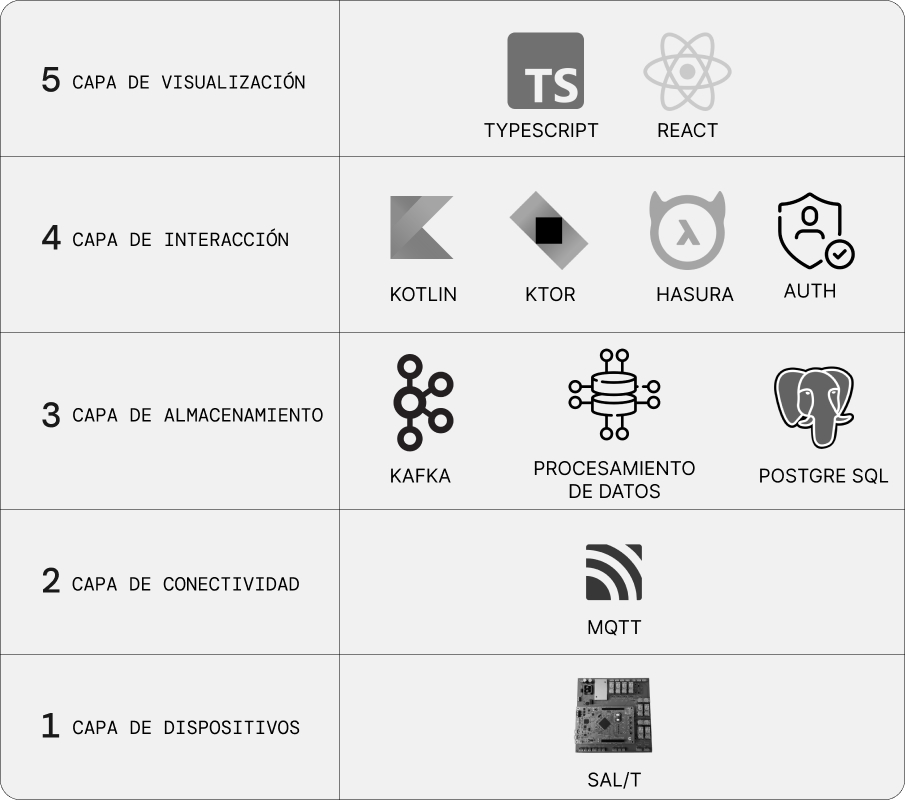
\includegraphics[width=.75\textwidth]{Figures/cuadro.jpg}
  \caption{Arquitectura de la Central Operativa SAL/T.}
  \label{fig:diagBloques}
\end{figure}



\subsection{Tecnologías del \textit{front-end}}

\subsubsection{TypeScript}

TypeScript es un lenguaje de programación de código abierto desarrollado por Microsoft que se basa en JavaScript. Es una extensión de JavaScript que agrega tipos estáticos opcionales y características de programación orientada a objetos avanzadas. TypeScript se compila a JavaScript y se puede usar en cualquier navegador o entorno de servidor que admita JavaScript. Permite una mayor seguridad y mantenibilidad en el código, lo que lo convierte en una opción popular para proyectos de gran escala y equipos de desarrollo. Además, se integra con muchos editores de código populares y frameworks, lo que facilita su adopción en proyectos existentes.


\newpage
\subsubsection{React}

React es una biblioteca de JavaScript de código abierto para construir interfaces de usuario (UI) interactivas y reutilizables. Fue desarrollado por Facebook y se ha convertido en una de las bibliotecas más populares para el desarrollo de aplicaciones web. React utiliza un enfoque basado en componentes para construir UI, lo que significa que los desarrolladores pueden crear piezas de UI reutilizables y componerlas para crear interfaces más complejas. React utiliza el DOM virtual para mejorar el rendimiento, lo que significa que solo actualiza las partes de la UI que necesitan ser actualizadas, en lugar de volver a dibujar toda la UI. React también se integra bien con otras bibliotecas y frameworks, lo que lo hace muy flexible y extensible.


\subsubsection{Parcel}

Parcel es una herramienta de construcción de código abierto que se utiliza para empaquetar y optimizar módulos de JavaScript y otros tipos de archivos. Ofrece una amplia gama de características útiles, como integración con hot module replacement (HMR), optimización de imágenes y capacidad de construcción paralela. Una de las principales ventajas de Parcel es su estrategia de "cero configuración", que hace que sea fácil de usar sin necesidad de una configuración adicional. Parcel también es altamente configurable y tiene una amplia compatibilidad con diferentes tecnologías y frameworks, como React, Vue y TypeScript. En general, Parcel es una herramienta de construcción rápida, fácil de usar y altamente personalizable que puede mejorar significativamente el flujo de trabajo del desarrollador.


\newpage
\subsubsection{Apollo}

Apollo es una plataforma de código abierto para el desarrollo de aplicaciones GraphQL. Ofrece una amplia gama de herramientas y servicios para ayudar a los desarrolladores a construir y mantener aplicaciones GraphQL de manera efectiva. Con Apollo, los desarrolladores pueden crear fácilmente clientes y servidores GraphQL, lo que les permite interactuar con diferentes fuentes de datos de manera eficiente. Además, Apollo tiene una amplia compatibilidad con diferentes frameworks y tecnologías, como React, Angular, Vue y Node.js. Apollo también ofrece características útiles, como la administración de caché, que pueden mejorar significativamente el rendimiento de las aplicaciones. En general, Apollo es una plataforma completa y fácil de usar que puede facilitar el proceso de desarrollo de aplicaciones GraphQL.


\subsubsection{Material UI}

Material UI es una biblioteca de componentes de interfaz de usuario de código abierto basada en el lenguaje de diseño Material Design de Google. Ofrece una amplia gama de componentes preconstruidos que se pueden utilizar para construir aplicaciones web modernas y atractivas. Los componentes de Material UI están altamente personalizados y pueden ser fácilmente adaptados a diferentes estilos y necesidades de diseño. Además, Material UI tiene una amplia compatibilidad con diferentes tecnologías y frameworks, como React, Angular y Vue. Material UI también ofrece características útiles, como soporte para temas personalizados y una interfaz de usuario responsiva que se adapta automáticamente a diferentes dispositivos. En general, Material UI es una biblioteca de componentes completa y fácil de usar que puede mejorar significativamente el proceso de desarrollo de aplicaciones web.


\subsubsection{JWT Decode}

JWT Decode es una biblioteca JavaScript de código abierto que se utiliza para decodificar tokens JSON Web Token (JWT). JWT Decode se puede utilizar para leer la información codificada en un token JWT, como el nombre de usuario y los roles de acceso. La biblioteca es fácil de usar y se puede integrar fácilmente en diferentes aplicaciones web y frameworks de JavaScript, como React y Angular. JWT Decode también ofrece características útiles, como la validación de tokens y la verificación de la firma, que pueden ayudar a garantizar la seguridad de la aplicación. En general, JWT Decode es una herramienta útil para decodificar y leer tokens JWT en aplicaciones de JavaScript.






%----------------------------------------------------------------------------------------
\newpage
\subsection{Tecnologías del \textit{backend}}


\subsubsection{Kotlin}


Kotlin es un lenguaje de programación de tipado estático, desarrollado por JetBrains, que puede correr sobre la máquina virtual de Java y también ser compilado en JavaScript y LLVM. Se caracteriza por ser un lenguaje moderno, conciso y seguro, que simplifica la programación en comparación con Java. Kotlin es utilizado en diversas aplicaciones, como Android, backend y frontend web, procesamiento de datos y desarrollo de aplicaciones para escritorio. Además, Kotlin cuenta con una gran comunidad de desarrolladores que lo respaldan, lo que ha llevado a que sea adoptado por empresas como Google, Netflix y Amazon. Otras de las características de Kotlin son su interoperabilidad con Java, soporte para programación funcional, orientación a objetos y manejo de nulos seguro. Kotlin ha ganado popularidad en los últimos años debido a su facilidad de uso, legibilidad y capacidad de reducir la cantidad de código necesaria para realizar tareas complejas.


\subsubsection{Ktor}

Ktor es un framework web de Kotlin que permite crear aplicaciones web y API REST de manera fácil y eficiente, con un enfoque en la programación funcional. Ktor es altamente modular y personalizable, lo que significa que los desarrolladores pueden seleccionar solo los componentes que necesitan para su aplicación, reduciendo así la complejidad y el tamaño del código. Algunas de las características de Ktor son su enfoque en la concurrencia y la eficiencia, soporte para diferentes tipos de autenticación y autorización, integración con librerías como Jackson y Koin, y facilidad para trabajar con bases de datos. Ktor es utilizado por empresas como JetBrains, Netflix y Pinterest, y ha ganado popularidad en la comunidad de desarrolladores de Kotlin debido a su facilidad de uso, alto rendimiento y capacidad de adaptarse a diferentes tipos de aplicaciones. Ktor es también compatible con diferentes plataformas, como Android y iOS, lo que lo hace ideal para proyectos que necesitan un backend escalable y eficiente.


\subsubsection{Kafka}

Kafka es una plataforma de streaming de datos, desarrollada por Apache, que permite a las aplicaciones enviar y recibir datos en tiempo real, de manera escalable, confiable y eficiente. Kafka se basa en el modelo de publicación/suscripción, en el que los productores envían mensajes a un "tema" y los consumidores reciben los mensajes de ese tema. Kafka se caracteriza por su alta velocidad y rendimiento, lo que lo hace ideal para aplicaciones que necesitan procesar grandes cantidades de datos en tiempo real, como análisis de datos, procesamiento de eventos y monitoreo de aplicaciones. Otras de las características de Kafka son su alta disponibilidad, escalabilidad horizontal, seguridad y facilidad para integrarse con otras herramientas y sistemas. 

\newpage
\subsubsection{Hasura}

Hasura es una plataforma de desarrollo de aplicaciones que permite a los desarrolladores crear, ejecutar y escalar aplicaciones con GraphQL de manera rápida y sencilla. Hasura se basa en una arquitectura sin servidor, lo que significa que los desarrolladores no tienen que preocuparse por el aprovisionamiento y la gestión de servidores, lo que reduce significativamente el tiempo de desarrollo. Hasura también ofrece una capa de seguridad de extremo a extremo, lo que permite a los desarrolladores proteger fácilmente sus datos y aplicaciones. Otras características de Hasura incluyen su facilidad para integrarse con diferentes bases de datos, incluyendo Postgres, MySQL y MongoDB, y su capacidad para generar automáticamente una API de GraphQL a partir de una base de datos existente. 


\subsubsection{PostgreSQL}

PostgreSQL es un sistema de gestión de bases de datos relacionales de código abierto y gratuito, utilizado por miles de empresas y organizaciones en todo el mundo. PostgreSQL se caracteriza por su fiabilidad, escalabilidad y seguridad, y es conocido por ser una de las bases de datos más poderosas y versátiles disponibles en la actualidad. PostgreSQL es compatible con una amplia gama de sistemas operativos y lenguajes de programación, y cuenta con una amplia variedad de herramientas y extensiones que hacen que sea fácil de usar y personalizar. Entre las características más destacadas de PostgreSQL se encuentran su soporte para transacciones ACID, su capacidad para manejar grandes volúmenes de datos y su integración con lenguajes de programación populares como Java, Python y PHP. 


\subsubsection{Mosquitto Broker}

Mosquitto es un broker MQTT de código abierto que se utiliza para transmitir mensajes entre dispositivos de Internet de las cosas (IoT) y otras aplicaciones. Mosquitto permite a los dispositivos conectarse y publicar o suscribirse a temas específicos, lo que permite una comunicación eficiente y en tiempo real. Es una herramienta popular en la industria del IoT debido a su escalabilidad y facilidad de uso. Mosquitto es compatible con una amplia variedad de plataformas, incluyendo Linux, Windows y macOS, y cuenta con una API de programación en C que permite a los desarrolladores integrar fácilmente la funcionalidad del broker MQTT en sus aplicaciones. Además, Mosquitto también tiene características de seguridad como autenticación y cifrado de datos, lo que lo hace adecuado para entornos de producción. Mosquitto es mantenido por la Eclipse Foundation y es utilizado por empresas como IBM, Amazon y Google en proyectos de IoT y M2M (machine-to-machine).


%----------------------------------------------------------------------------------------
\newpage
\subsection{Tecnologías del \textit{firmware}}


\subsubsection{C lang}

C es un lenguaje de programación de propósito general que se utiliza ampliamente en el desarrollo de sistemas operativos, aplicaciones de bajo nivel y dispositivos embebidos. Fue desarrollado originalmente en la década de 1970 y ha sido una de las lenguas de programación más influyentes en la historia de la informática. C es conocido por ser un lenguaje de programación estructurado que permite a los desarrolladores escribir código claro y legible, con una sintaxis simple y directa. Ofrece un gran control sobre la memoria y la capacidad de acceder directamente al hardware. C es también un lenguaje de programación portátil, lo que significa que el código escrito en C puede ser compilado en diferentes plataformas y sistemas operativos. C se ha utilizado para crear algunos de los sistemas operativos y programas más importantes del mundo, como Unix, el kernel de Linux y la mayoría de los sistemas operativos de Apple. Es un lenguaje de programación esencial para cualquier persona que busque una carrera en la programación de sistemas y aplicaciones de bajo nivel.


\subsubsection{FreeRTOS}

FreeRTOS es un sistema operativo en tiempo real (RTOS) de código abierto y gratuito que se utiliza para controlar sistemas embebidos y microcontroladores. Es ampliamente utilizado en aplicaciones de control industrial, automoción, electrónica de consumo y aeroespacial, debido a su capacidad para proporcionar un rendimiento confiable y predecible en tiempo real. FreeRTOS es conocido por ser altamente portátil, lo que permite a los desarrolladores escribir código que se puede compilar para diferentes plataformas y arquitecturas de hardware. Ofrece una variedad de funcionalidades, como gestión de tareas, semáforos, colas y temporizadores, lo que permite a los desarrolladores crear sistemas complejos con una gestión eficiente de los recursos. FreeRTOS es fácil de usar y cuenta con una gran comunidad de desarrolladores que ofrecen soporte y recursos. Es una opción popular para proyectos de sistemas embebidos que requieren una solución RTOS de alto rendimiento y confiabilidad.


\subsubsection{Paho MQTT \textit{client}}

 Paho MQTT es una biblioteca de código abierto para implementar el protocolo MQTT (Message Queuing Telemetry Transport) en aplicaciones de IoT y sistemas embebidos. La biblioteca Paho proporciona una API consistente para programar clientes MQTT en diferentes plataformas, como Java, C, C++, Python, Javascript, entre otras. Paho MQTT permite la conexión y la comunicación bidireccional entre dispositivos IoT y aplicaciones, lo que facilita la implementación de soluciones de IoT en diferentes contextos. La biblioteca es altamente configurable y permite ajustar varios parámetros, como la calidad de servicio, la retención de mensajes y los tiempos de espera. Paho MQTT también proporciona herramientas para monitorear y depurar las comunicaciones MQTT, lo que facilita la identificación y solución de problemas en el sistema. La biblioteca se mantiene activamente y cuenta con una gran comunidad de desarrolladores que contribuyen a su mejora y ofrecen soporte.


%----------------------------------------------------------------------------------------
\section{Herramientas utilizadas}


\subsubsection{Docker}

Docker es una plataforma de software libre que permite crear, distribuir y ejecutar aplicaciones en contenedores de software. Los contenedores de Docker encapsulan aplicaciones y todas sus dependencias en un paquete independiente que se puede ejecutar en cualquier entorno, independientemente del sistema operativo o la infraestructura subyacente. Docker utiliza tecnologías como el kernel de Linux y las redes virtuales para garantizar que los contenedores sean livianos y portables. Los contenedores de Docker se ejecutan en un entorno aislado y seguro, lo que ayuda a prevenir conflictos entre aplicaciones y mejora la seguridad de los sistemas. Docker es una herramienta esencial para la creación y el despliegue de aplicaciones en la nube, ya que facilita el proceso de implementación y mejora la escalabilidad y la eficiencia de los sistemas. La plataforma cuenta con una gran comunidad de desarrolladores que contribuyen con plugins y herramientas adicionales, y que ofrecen soporte y documentación para su uso.

\subsubsection{Docker Compose}

Docker Compose es la herramienta que permite ejecutar aplicaciones multi-contenedor en Docker se utiliza para definir las relaciones entre los contenedores de la aplicación. Con ella, es posible crear un archivo YAML que especifica la configuración de cada servicio, las redes y volúmenes que se utilizarán para comunicar y almacenar datos entre los contenedores. Gracias a esto, podemos coordinar eficientemente múltiples servicios como bases de datos, servidores web, balanceadores de carga, etc. en una o varias máquinas. 


\subsubsection{Redpanda}

Redpanda es una plataforma de streaming de datos de alta velocidad que ofrece una alternativa escalable y confiable a los sistemas de streaming de datos existentes. Permite el procesamiento en tiempo real de grandes cantidades de datos, lo que lo hace ideal para su uso en aplicaciones de transmisión de datos en vivo, análisis de datos, aprendizaje automático y más. Además, Redpanda es altamente resistente a fallos, lo que significa que puede manejar situaciones inesperadas y garantizar la continuidad del servicio en todo momento. También ofrece herramientas integradas de monitoreo y gestión, lo que facilita la administración de la plataforma de manera eficiente.


\subsubsection{Git}

Git es un sistema de control de versiones de software de código abierto que permite a los desarrolladores rastrear y administrar los cambios en el código fuente de sus proyectos. Con Git, los desarrolladores pueden colaborar en proyectos de software de manera efectiva, ya que pueden trabajar en diferentes versiones del código simultáneamente y fusionar los cambios de manera transparente. Git utiliza una estructura de árbol para registrar los cambios en el código y tiene una gran cantidad de características avanzadas, como la creación de ramas, el etiquetado y la reversión de cambios. Git es una herramienta esencial para la gestión de proyectos de software y es utilizado por millones de desarrolladores en todo el mundo.


\subsubsection{MQTT.fx}

MQTT.fx es una herramienta de escritorio gratuita y de código abierto para la visualización y la prueba de clientes MQTT. Esta aplicación permite a los usuarios conectarse a brokers MQTT y suscribirse a diferentes temas para recibir mensajes en tiempo real. Además, MQTT.fx proporciona una interfaz gráfica de usuario intuitiva para la publicación de mensajes MQTT y la configuración de parámetros avanzados de MQTT. Es una herramienta útil para los desarrolladores y administradores de sistemas que necesitan depurar y probar aplicaciones MQTT, así como para aquellos que desean explorar y aprender sobre el protocolo MQTT.


\subsubsection{CLion}

CLion es un entorno de desarrollo integrado (IDE) multiplataforma y de alta calidad para el lenguaje de programación C y C++. Ofrece una amplia gama de características avanzadas, como la integración con herramientas externas, el depurador avanzado, la finalización automática de código y la refactorización de código inteligente. CLion también admite múltiples sistemas de construcción y está diseñado para trabajar con una variedad de herramientas populares, como CMake, Makefile y otros.


\subsubsection{Wireshark}

Wireshark es una herramienta de análisis de redes de código abierto y gratuita que permite capturar y analizar el tráfico de red en tiempo real. Con Wireshark, los usuarios pueden ver el tráfico de red en detalle y analizar protocolos en profundidad, lo que facilita la resolución de problemas en redes de datos y la detección de vulnerabilidades de seguridad. Ofrece una interfaz de usuario gráfica y es compatible con diferentes plataformas, como Windows, Mac y Linux. Es una herramienta útil para los profesionales de redes y seguridad, así como para los entusiastas de la tecnología que desean profundizar en el análisis de redes.


\subsubsection{Herramientas del navegador de internet}

Las herramientas del navegador de Internet son fundamentales para el desarrollo web. La consola es una herramienta útil para ver y depurar errores en el código JavaScript, y también para interactuar con la página en tiempo real. La pestaña de red es esencial para el análisis de la carga de recursos de la página, permitiendo ver las solicitudes HTTP y el tiempo de carga de cada recurso. Por último, la pestaña de aplicación permite ver y modificar los datos almacenados en el almacenamiento local y las cookies de la página web.


\subsubsection{JTAG}

JTAG (Joint Test Action Group) es un estándar para la depuración y programación de dispositivos electrónicos. Permite acceder a los pines de prueba de un dispositivo para realizar pruebas de hardware y depuración a nivel de circuito. JTAG se utiliza en una amplia variedad de dispositivos, desde chips integrados en dispositivos móviles hasta procesadores de computadoras de escritorio. También se utiliza en la programación de dispositivos de Internet de las cosas (IoT) y en la depuración de tarjetas electrónicas. JTAG se ha convertido en un estándar común para la depuración y programación de dispositivos, y muchas herramientas de desarrollo de software y hardware lo admiten.


\subsubsection{ST-Link}

ST-Link es una herramienta de programación y depuración de microcontroladores fabricada por STMicroelectronics. Se utiliza para programar y depurar microcontroladores STM32 y otros dispositivos compatibles con JTAG o SWD. La herramienta se conecta al ordenador mediante USB y se puede usar con una variedad de entornos de desarrollo integrados (IDE) y herramientas de depuración. ST-Link es una opción popular y accesible para los desarrolladores que trabajan con microcontroladores STM32.


\subsubsection{STM32CubeMX}

STM32CubeMX es una herramienta de software que permite la configuración rápida y fácil de los microcontroladores STM32 de STMicroelectronics. Con esta herramienta se puede generar código inicial para proyectos y configurar periféricos de manera visual. Además, incluye un amplio conjunto de ejemplos de código y documentación para ayudar en el desarrollo de proyectos. STM32CubeMX también ofrece una integración sencilla con el entorno de desarrollo integrado (IDE) de STM32, lo que facilita el flujo de trabajo para los desarrolladores.


\subsubsection{STM32CubeProgrammer - SWV}

STM32CubeProgrammer es una herramienta de programación y depuración de microcontroladores STM32 de STMicroelectronics. Además de la programación y el borrado de la memoria flash, también es capaz de programar la memoria RAM y de configurar las opciones de protección de la memoria. SWV (Serial Wire Viewer) es una de las características más destacadas de STM32CubeProgrammer, que permite el monitoreo en tiempo real del comportamiento del microcontrolador a través de la línea de depuración SWD (Serial Wire Debug). SWV es útil para depurar y optimizar el código, ya que permite visualizar la ejecución de instrucciones, la utilización de la memoria y el uso de interrupciones en tiempo real.


